\documentclass[11pt]{article}
\usepackage{amssymb,amsmath,amsthm,latexsym,mathrsfs,array,amssymb,amsmath,epsfig,sudoku,amssymb,amsbsy,array,color,amssymb,amsmath,epsfig,sudoku,url}
\usepackage{minted}
\usepackage{pdflscape}
\usemintedstyle{vs}
\usepackage{booktabs}
\usepackage{float}

\usepackage{amsmath} % For advanced math features like \text, \frac, etc.
\usepackage[utf8]{inputenc} % To handle various characters
\usepackage{float}
\usepackage{booktabs}
%\usepackage[a4paper, margin=0.5in]{geometry}

\textheight 8.5in
\textwidth 6.25in
\voffset= -.55in
\hoffset= -.55in

\date{}
\pagestyle{empty}
\begin{document}
%\begin{landscape}
%\thispagestyle{empty}
\begin{center} {\LARGE\textbf{{CSCI 6360}}}\end{center}
\begin{center}{\Large \textbf{Project 3}}\end{center}
%\begin{center}{Masum Billah \\ University of GA \\ Department of Statistics}\end{center}       
\begin{center} \date{\today} \today \end{center}
    
\vspace{.1in}

\section{Model}
\begin{minted}{python}
class NN(nn.Module):
    def __init__(self, input_dim, version="m1"):
        super().__init__()

        if version == "m1":
            self.mlp = nn.Sequential(
                nn.Linear(input_dim, 64),
                nn.ReLU(),
                nn.Linear(64, 64),
                nn.ReLU(),
                nn.Linear(64, 64),
                nn.ReLU(),
                nn.Linear(64, 1)
            )
        elif version == "m2":
            self.mlp = nn.Sequential(
                nn.Linear(input_dim, 128),
                nn.ReLU(),
                nn.Linear(128, 128),
                nn.ReLU(),
                nn.Linear(128, 64),
                nn.ReLU(),
                nn.Linear(64, 1)
            )
        elif version == "m3": 
            self.mlp = nn.Sequential(
                nn.Linear(input_dim, 128),
                nn.ReLU(),
                nn.Linear(128, 64),
                nn.ReLU(),
                nn.Linear(64, 32),
                nn.ReLU(),
                nn.Linear(32, 1)
            )
    def forward(self, x):
        return self.mlp(x)
\end{minted}

\section{In-sample regression performance on Dataset 1.}

\begin{table}[H]
\centering
\caption{In-sample regression performance on the Insurance Charges dataset using a learning rate of $0.01$.}
\label{tab:California_Housing_(In-Sample)}
\begin{tabular}{lrrr}
\toprule
 & $model_1$ & $model_2$ & $model_3$ \\
\midrule
r2 & 0.872 & 0.890 & 0.879 \\
sst & 196074242048.000 & 196074242048.000 & 196074242048.000 \\
sse & 25073192960.000 & 21539094528.000 & 23702245376.000 \\
mse & 18739307.145 & 16097977.973 & 17714682.643 \\
rmse & 4328.892 & 4012.229 & 4208.881 \\
mae & 2590.035 & 2220.552 & 2397.691 \\
n & 1338.000 & 1338.000 & 1338.000 \\
aic & 45448.327 & 45245.045 & 45373.092 \\
bic & 105345.214 & 105141.932 & 105269.979 \\
\bottomrule
\end{tabular}
\end{table}


\begin{table}[H]
\centering
\caption{In-sample regression performance on the Insurance Charges dataset using a learning rate of $0.03$.}
\label{tab:Auto_MPG_(In-Sample)}
\begin{tabular}{lrrr}
\toprule
 & model$_1$ & model$_2$ & model$_3$ \\
\midrule
r2 & 0.896 & 0.943 & 0.899 \\
sst & 196074242048.000 & 196074242048.000 & 196074242048.000 \\
sse & 20436989952.000 & 11249342464.000 & 19720007680.000 \\
mse & 15274282.475 & 8407580.317 & 14738421.286 \\
rmse & 3908.233 & 2899.583 & 3839.065 \\
mae & 2362.465 & 1697.792 & 2307.006 \\
n & 1338.000 & 1338.000 & 1338.000 \\
aic & 45174.769 & 44375.934 & 45126.986 \\
bic & 105071.656 & 104272.821 & 105023.872 \\
\bottomrule
\end{tabular}
\end{table}


\begin{table}[H]
\centering
\caption{In-sample regression performance on the Insurance Charges dataset using a learning rate of $0.05$.}
\label{tab:Auto_MPG_(In-Sample)}
\begin{tabular}{lrrr}
\toprule
 & model$_1$ & model$_2$ & model$_3$ \\
\midrule
r2 & 0.901 & 0.943 & 0.923 \\
sst & 196074242048.000 & 196074242048.000 & 196074242048.000 \\
sse & 19318460416.000 & 11204450304.000 & 15181498368.000 \\
mse & 14438311.223 & 8374028.628 & 11346411.336 \\
rmse & 3799.778 & 2893.791 & 3368.443 \\
mae & 2697.286 & 1704.748 & 2080.025 \\
n & 1338.000 & 1338.000 & 1338.000 \\
aic & 45099.459 & 44370.584 & 44777.023 \\
bic & 104996.346 & 104267.471 & 104673.910 \\
\bottomrule
\end{tabular}
\end{table}

\begin{figure}[h]
\centering
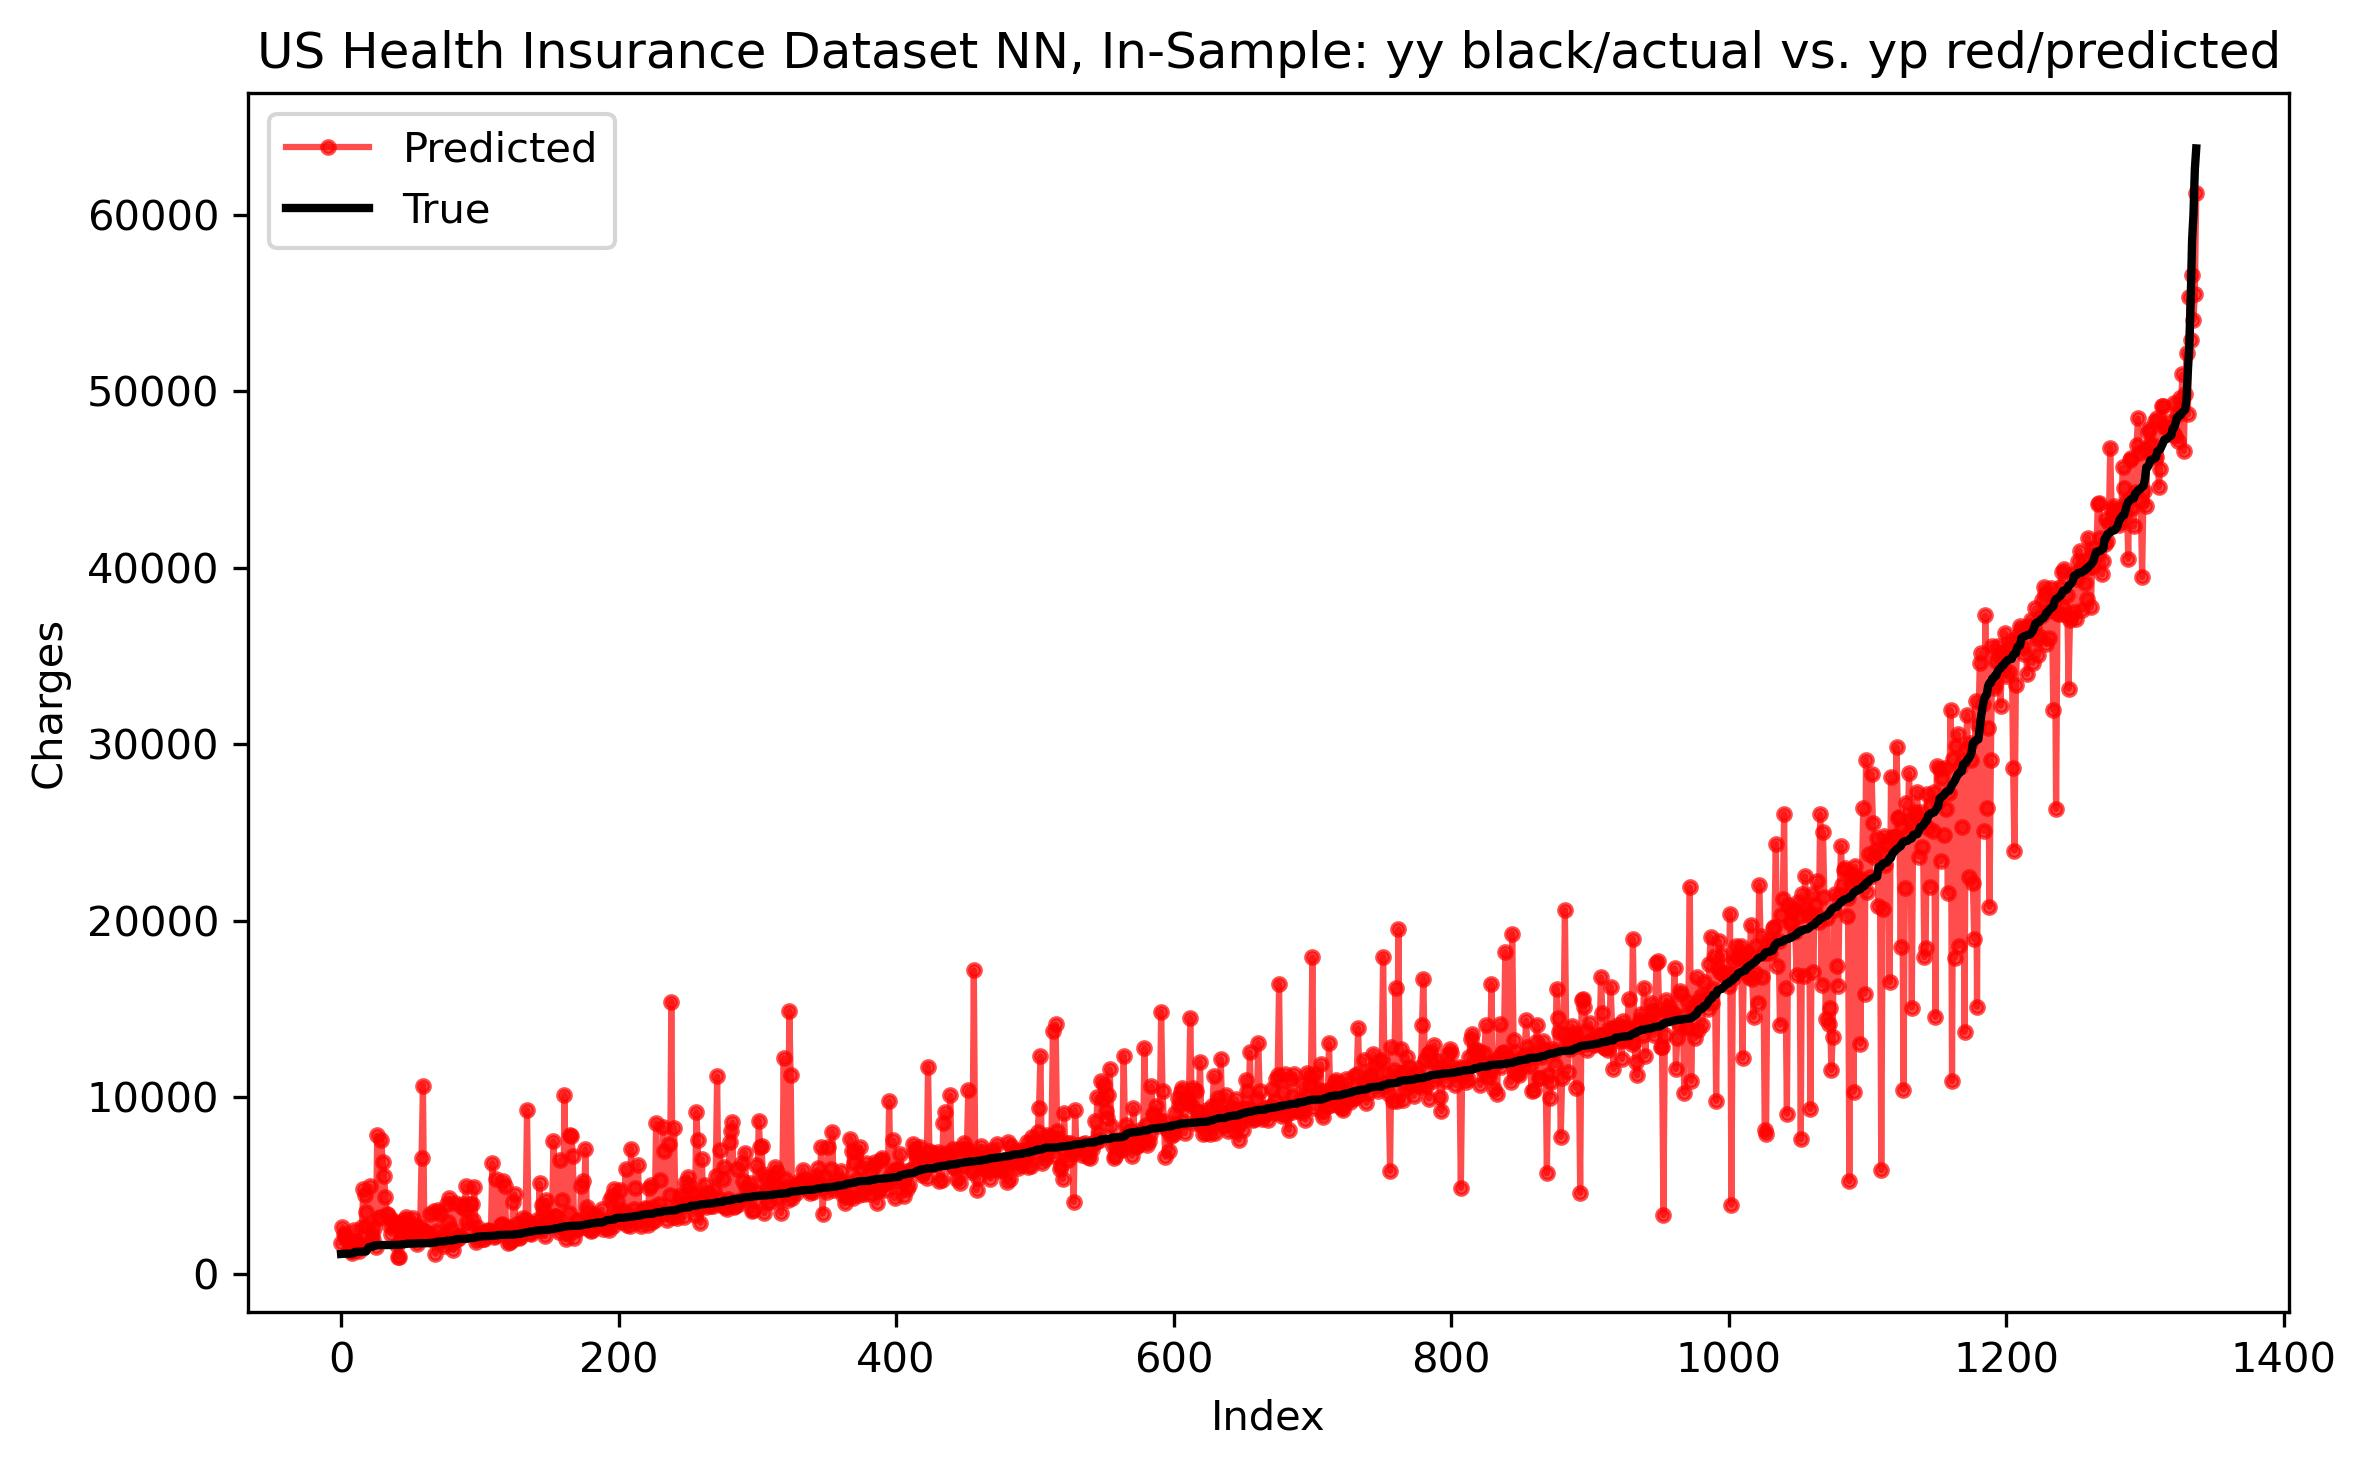
\includegraphics[width=0.9\textwidth]{figure/insurance_in_sample_0.05.jpg}

\caption{In-sample performance of a multi-layer neural network (Model 2) on the Insurance Charges dataset with a fine-tuned learning rate of $0.05$.}

\label{fig:cnn1}
\end{figure}


\section{Out-of-sample regression performance on Dataset 1}


\begin{table}[H]
\centering
\caption{Out-of-sample regression performance on the Insurance Charges dataset using a learning rate of $0.01$.}
\label{tab:Auto_MPG_(In-Sample)}
\begin{tabular}{lrrr}
\toprule
 & model$_1$ & model$_2$ & model$_3$ \\
\midrule
r2 & 0.844 & 0.857 & 0.847 \\
sst & 41606660096.000 & 41606660096.000 & 41606660096.000 \\
sse & 6479005184.000 & 5932235776.000 & 6378529792.000 \\
mse & 24175392.478 & 22135208.119 & 23800484.299 \\
rmse & 4916.848 & 4704.807 & 4878.574 \\
mae & 3191.396 & 2447.520 & 2853.070 \\
n & 268.000 & 268.000 & 268.000 \\
aic & 27598.227 & 27574.598 & 27594.038 \\
bic & 68969.988 & 68946.359 & 68965.799 \\
\bottomrule
\end{tabular}

\end{table}


\begin{table}[H]
\centering
\caption{Out-of-sample regression performance on the Insurance Charges dataset using a learning rate of $0.03$.}
\label{tab:Auto_MPG_(In-Sample)}
\begin{tabular}{lrrr}
\toprule
 & model$_1$ & model$_2$ & model$_3$ \\
\midrule
r2 & 0.849 & 0.829 & 0.833 \\
sst & 41606660096.000 & 41606660096.000 & 41606660096.000 \\
sse & 6284380160.000 & 7101800448.000 & 6937900544.000 \\
mse & 23449179.701 & 26499255.403 & 25887688.597 \\
rmse & 4842.435 & 5147.743 & 5087.995 \\
mae & 2776.404 & 2935.075 & 2804.652 \\
n & 268.000 & 268.000 & 268.000 \\
aic & 27590.053 & 27622.824 & 27616.567 \\
bic & 68961.814 & 68994.585 & 68988.328 \\
\bottomrule
\end{tabular}
\end{table}


\begin{table}[H]
\centering
\caption{Out-of-sample regression performance on the Insurance Charges dataset using a learning rate of $0.05$.}
\label{tab:Auto_MPG_(In-Sample)}

\begin{tabular}{lrrr}
\toprule
 & model$_1$ & model$_2$ & model$_3$ \\
\midrule
r2 & 0.809 & 0.820 & 0.811 \\
sst & 41606660096.000 & 41606660096.000 & 41606660096.000 \\
sse & 7938720768.000 & 7486139392.000 & 7878475776.000 \\
mse & 29622092.418 & 27933355.940 & 29397297.672 \\
rmse & 5442.618 & 5285.202 & 5421.927 \\
mae & 2930.985 & 2848.854 & 2918.611 \\
n & 268.000 & 268.000 & 268.000 \\
aic & 27652.680 & 27636.949 & 27650.639 \\
bic & 69024.441 & 69008.710 & 69022.400 \\
\bottomrule
\end{tabular}
\end{table}


\begin{figure}[h]
\centering
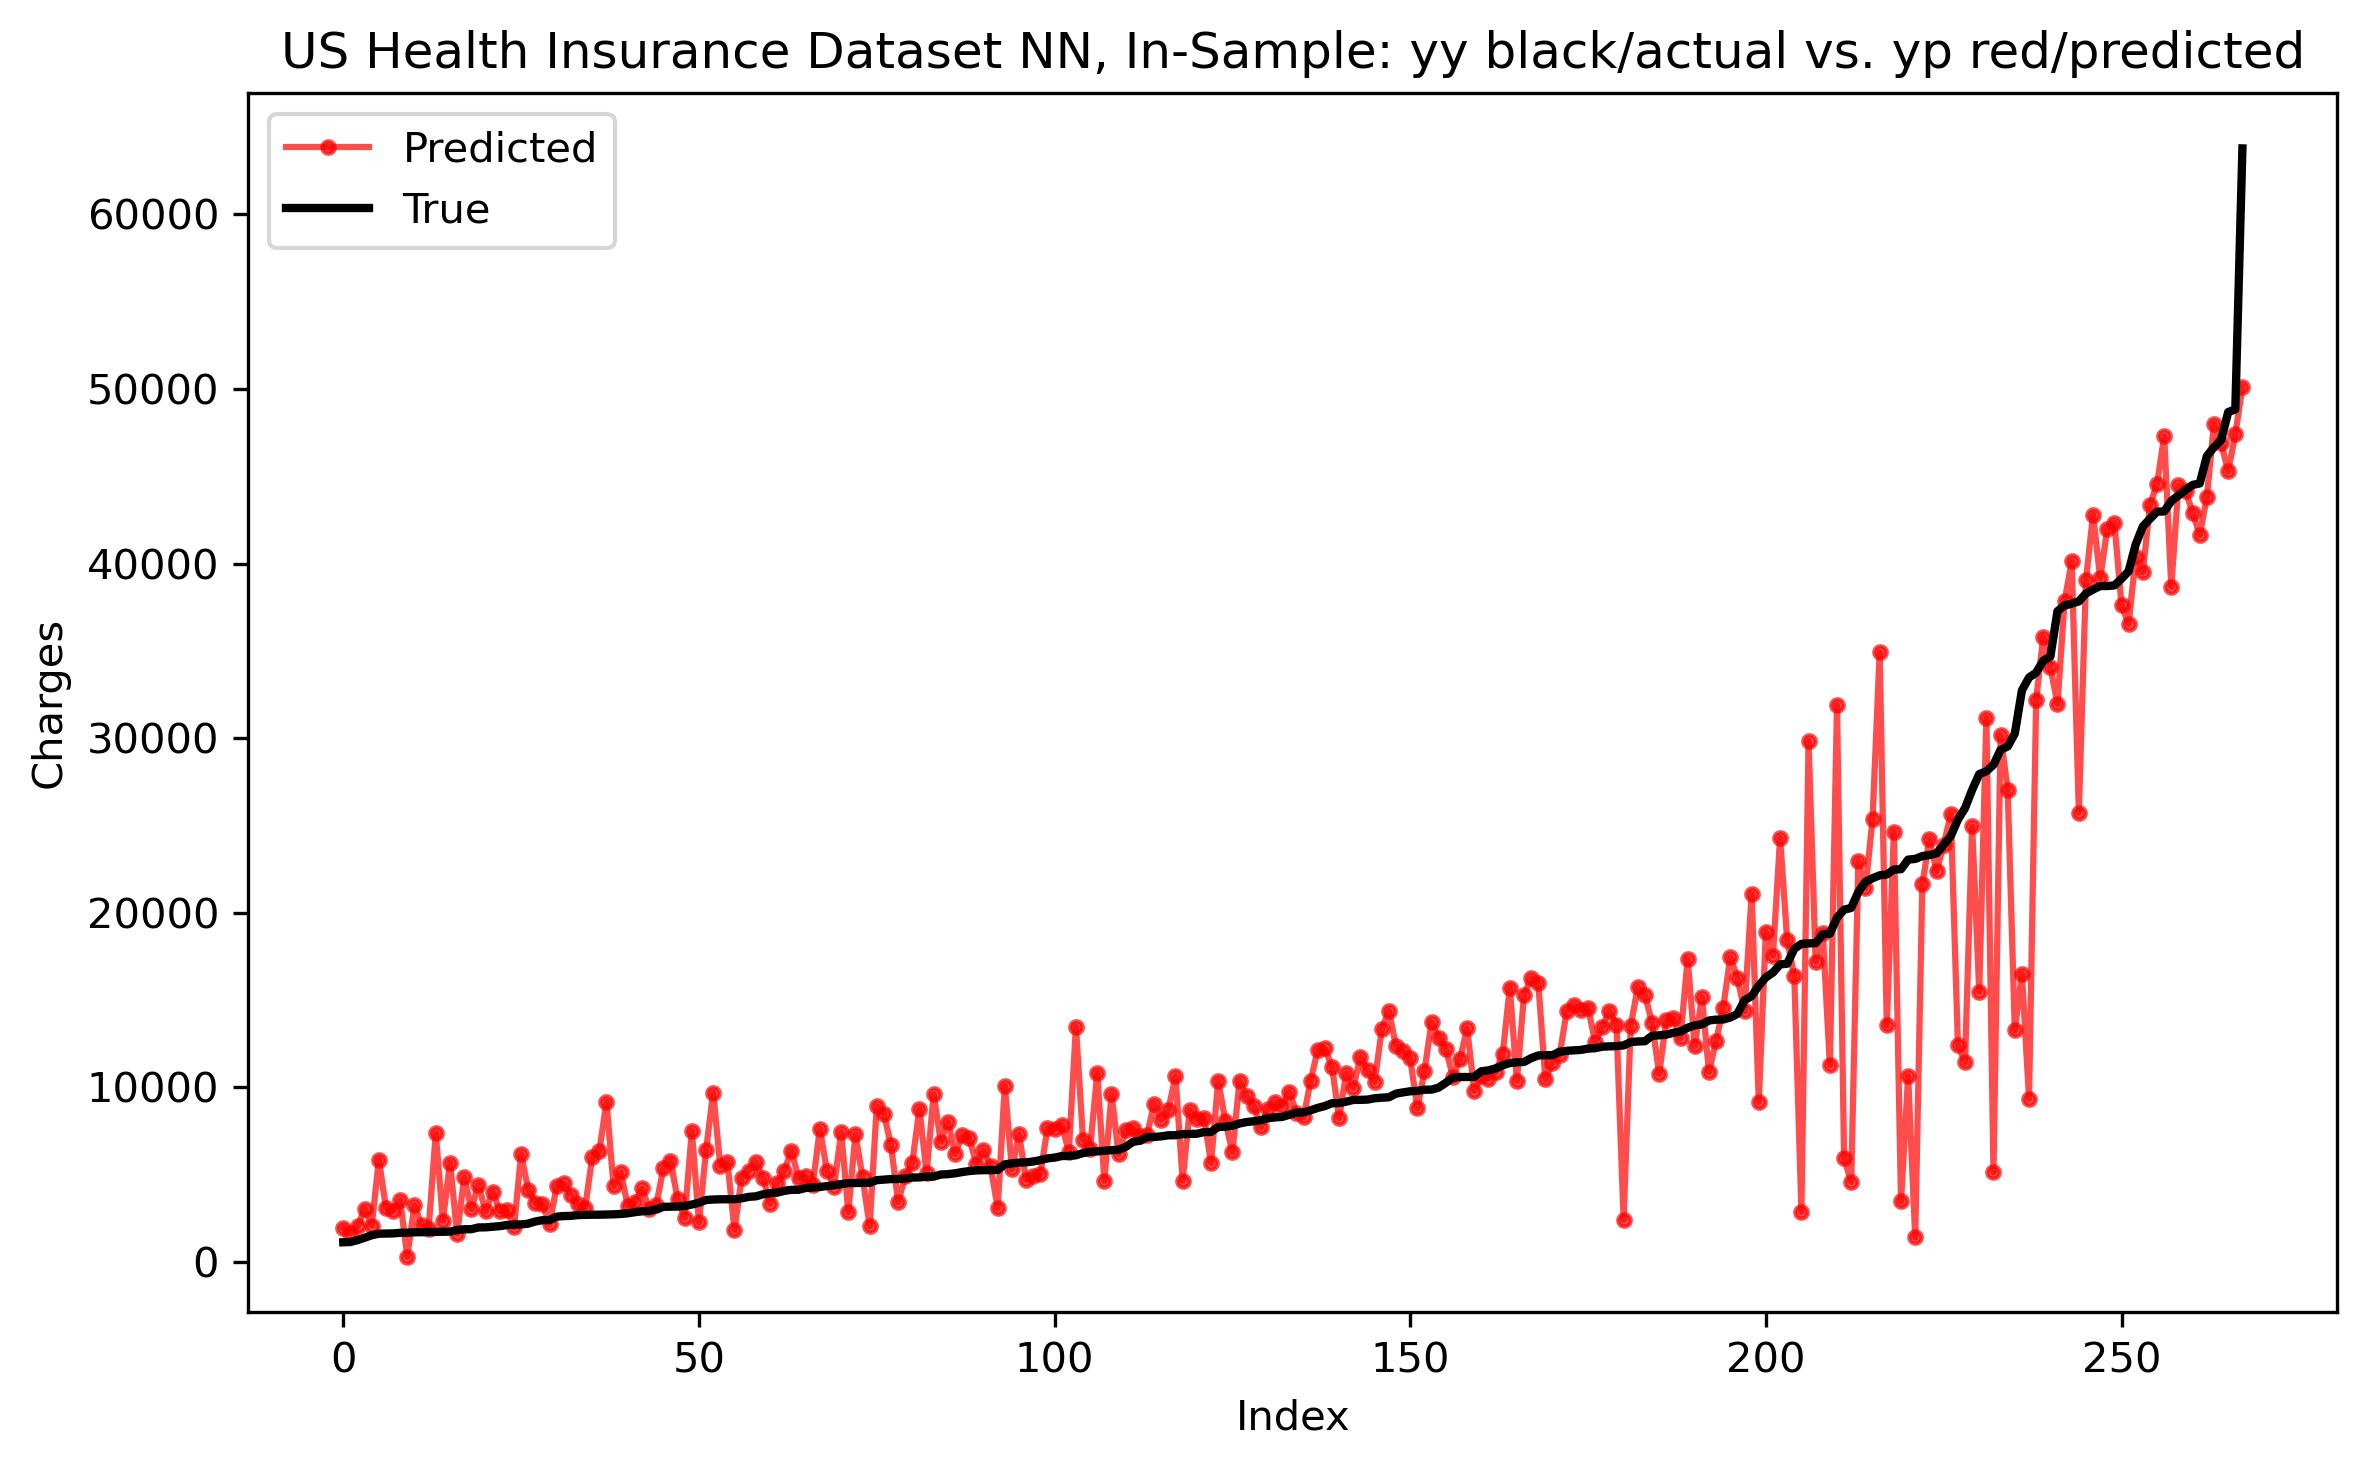
\includegraphics[width=0.9\textwidth]{figure/insurance_out_sample_0.01.jpg}

\caption{Out-of-sample performance of a multi-layer neural network (Model 2) on the Insurance Charges dataset with a fine-tuned learning rate of $0.01$.}

\label{fig:cnn1}
\end{figure}




\section{In-sample regression performance on Dataset 2}

\begin{table}[H]
\centering
\caption{In-sample regression performance on the Insurance Charges dataset using a learning rate of $0.01$.}
\label{tab:Auto_MPG_(In-Sample)}
\begin{tabular}{lrrr}
\toprule
 & model$_1$ & model$_2$ & model$_3$ \\
\midrule
r2 & 0.872 & 0.891 & 0.875 \\
sst & 196074225664.000 & 196074225664.000 & 196074225664.000 \\
sse & 25085812736.000 & 21277478912.000 & 24470661120.000 \\
mse & 18748738.966 & 15902450.607 & 18288984.395 \\
rmse & 4329.981 & 3987.788 & 4276.562 \\
mae & 2636.714 & 2235.030 & 2408.875 \\
n & 1338.000 & 1338.000 & 1338.000 \\
aic & 45449.000 & 45228.694 & 45415.781 \\
bic & 105345.887 & 105125.581 & 105312.668 \\
\bottomrule
\end{tabular}
\end{table}

\begin{table}[H]
\centering
\caption{In-sample regression performance on the Insurance Charges dataset using a learning rate of $0.03$.}
\label{tab:Auto_MPG_(In-Sample)}
\begin{tabular}{lrrr}
\toprule
 & model$_1$ & model$_2$ & model$_3$ \\
\midrule
r2 & 0.895 & 0.929 & 0.919 \\
sst & 196074225664.000 & 196074225664.000 & 196074225664.000 \\
sse & 20505407488.000 & 13916065792.000 & 15851454464.000 \\
mse & 15325416.658 & 10400647.079 & 11847125.907 \\
rmse & 3914.769 & 3225.003 & 3441.965 \\
mae & 2219.960 & 2130.200 & 2152.952 \\
n & 1338.000 & 1338.000 & 1338.000 \\
aic & 45179.241 & 44660.573 & 44834.803 \\
bic & 105076.128 & 104557.459 & 104731.690 \\
\bottomrule
\end{tabular}

\end{table}


\begin{table}[H]
\centering
\caption{In-sample regression performance on the Insurance Charges dataset using a learning rate of $0.05$.}
\label{tab:Auto_MPG_(In-Sample)}
\begin{tabular}{lrrr}
\toprule
 & model$_1$ & model$_2$ & model$_3$ \\
\midrule
r2 & 0.926 & 0.935 & 0.930 \\
sst & 196074225664.000 & 196074225664.000 & 196074225664.000 \\
sse & 14436622336.000 & 12748170240.000 & 13750960128.000 \\
mse & 10789702.792 & 9527780.448 & 10277249.722 \\
rmse & 3284.768 & 3086.710 & 3205.815 \\
mae & 1844.827 & 1830.518 & 1818.018 \\
n & 1338.000 & 1338.000 & 1338.000 \\
aic & 44709.710 & 44543.289 & 44644.603 \\
bic & 104606.596 & 104440.175 & 104541.490 \\
\bottomrule
\end{tabular}
\end{table}

\begin{figure}[h]
\centering
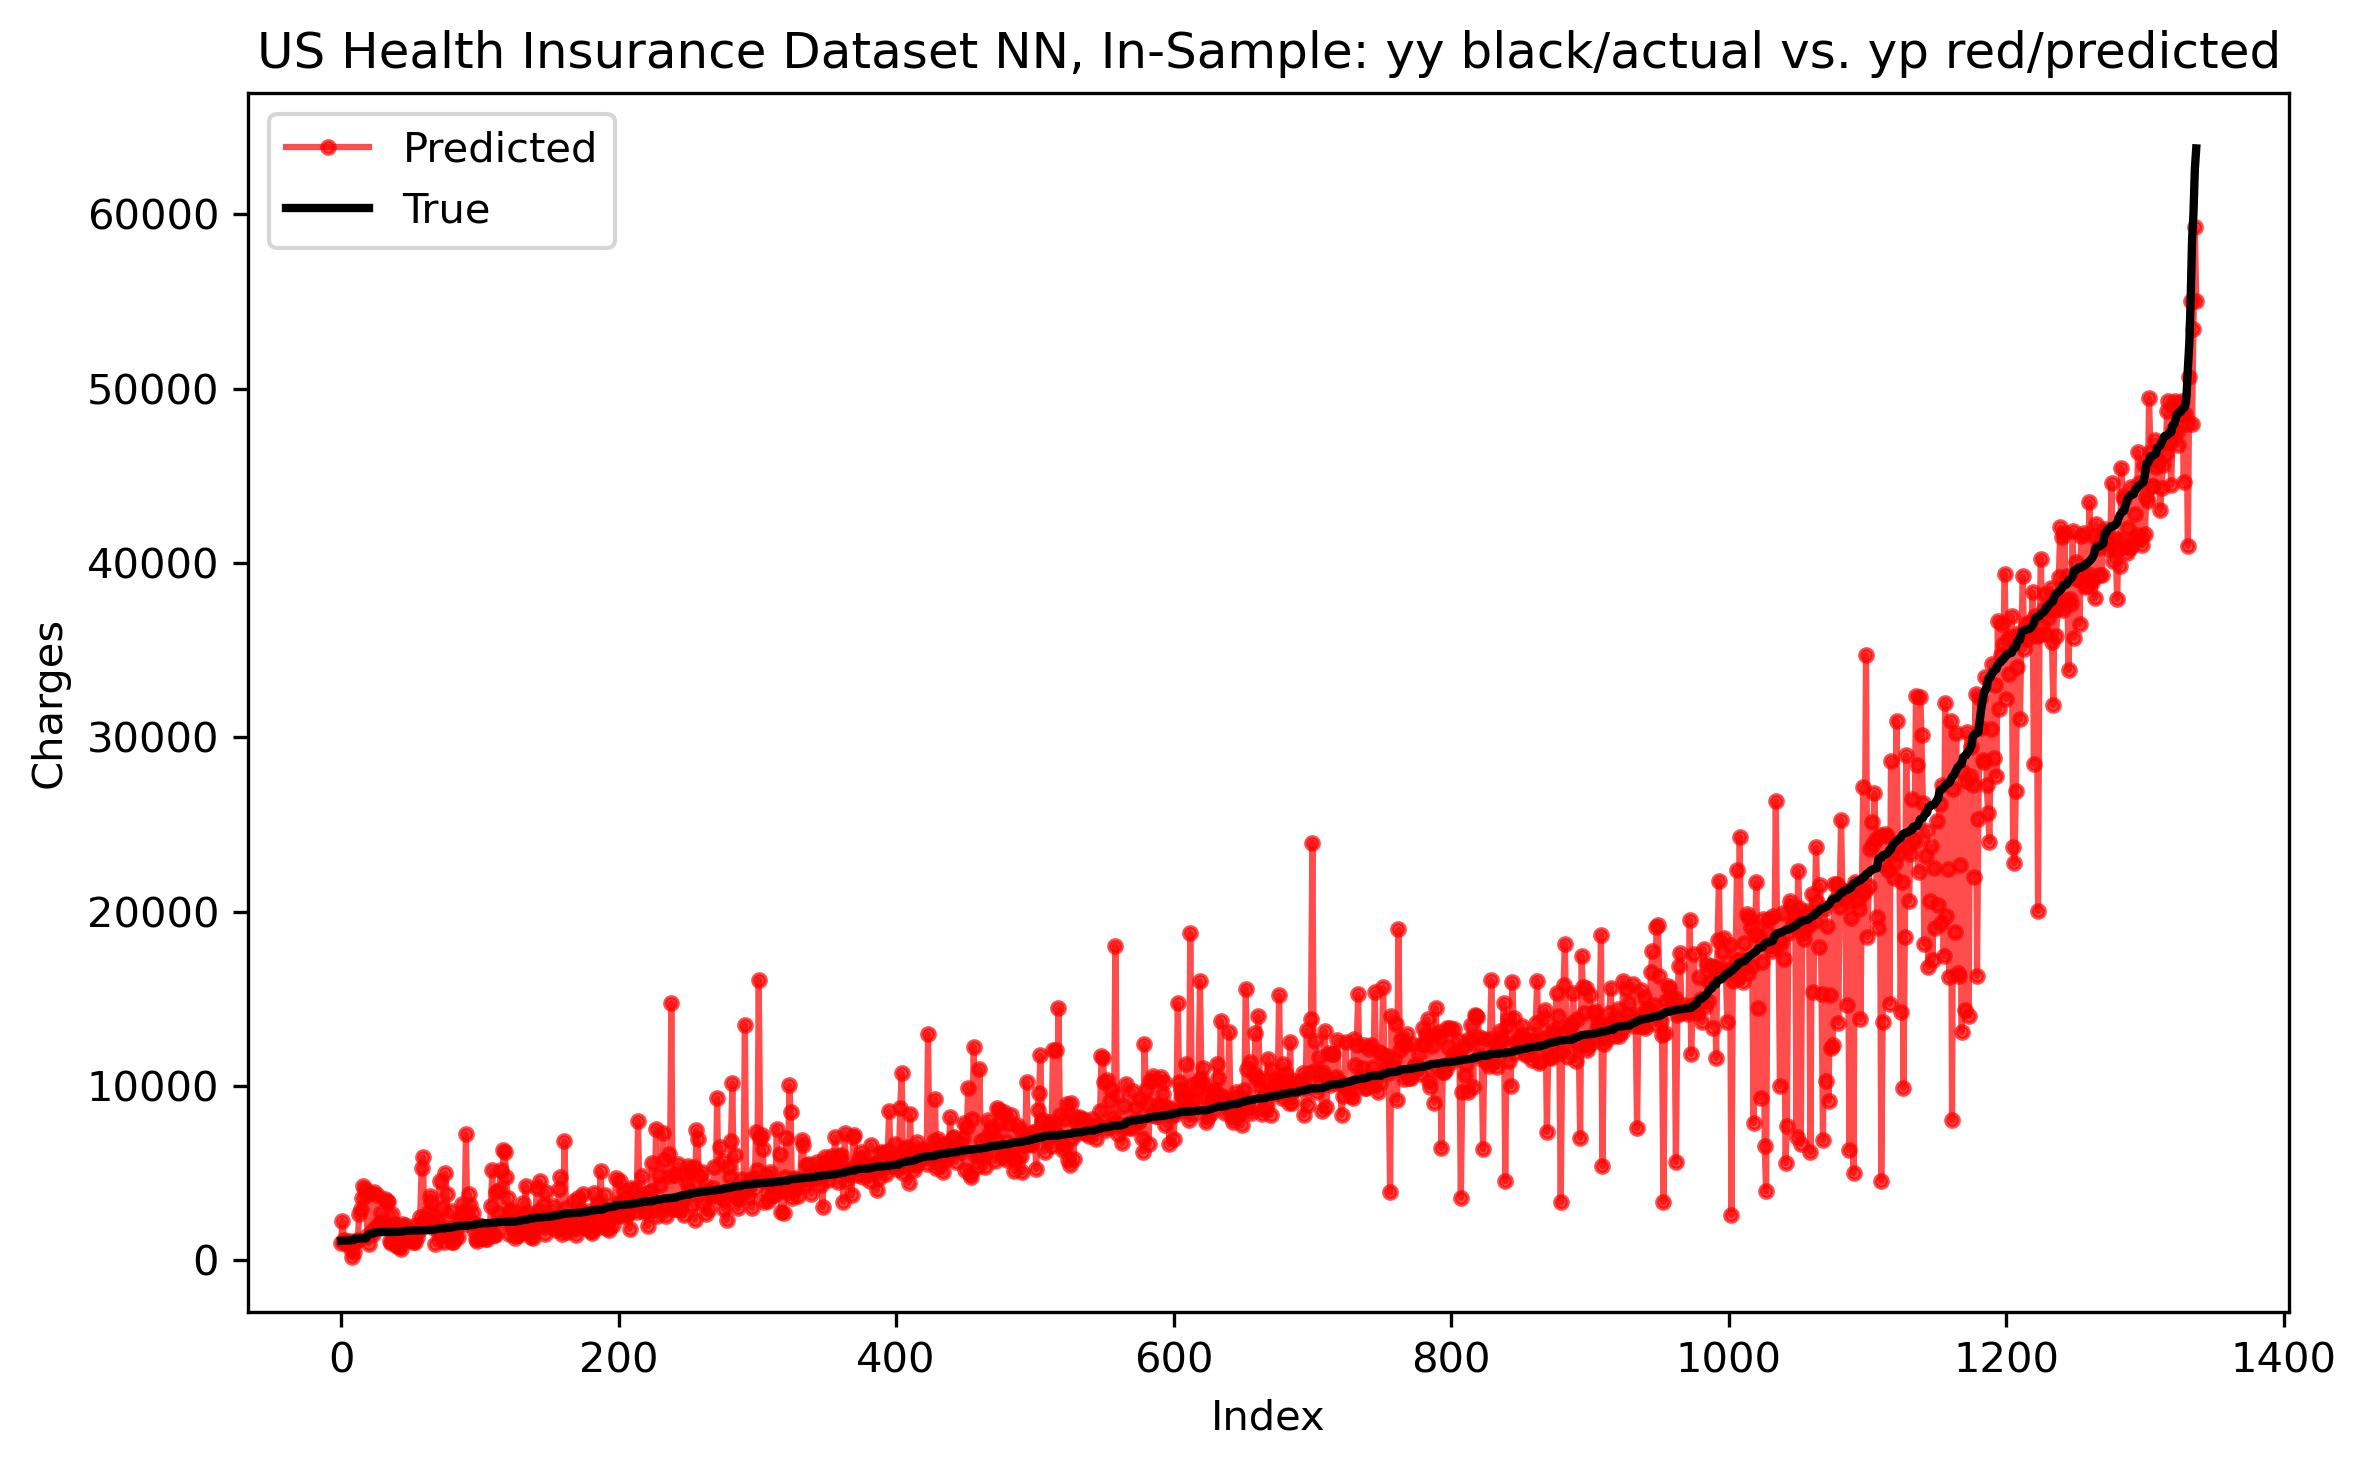
\includegraphics[width=0.9\textwidth]{figure/medical_in_sample_0.05.jpg}
\caption{In-sample performance of a multi-layer neural network (Model 2) on the Insurance Charges dataset with a fine-tuned learning rate of $0.05$.}


\label{fig:cnn1}
\end{figure}
\newpage

\section{Out-of-sample regression performance on Dataset 2}

\begin{table}[H]
\centering
\caption{Out-of-sample regression performance on the Insurance Charges dataset using a learning rate of $0.01$.}
\label{tab:Auto_MPG_(In-Sample)}
\begin{tabular}{lrrr}
\toprule
 & model$_1$ & model$_2$ & model$_3$ \\
\midrule
r2 & 0.855 & 0.846 & 0.845 \\
sst & 41606660096.000 & 41606660096.000 & 41606660096.000 \\
sse & 6046942208.000 & 6411969024.000 & 6435321344.000 \\
mse & 22563217.194 & 23925257.552 & 24012393.075 \\
rmse & 4750.075 & 4891.345 & 4900.244 \\
mae & 3058.983 & 2703.244 & 3008.303 \\
n & 268.000 & 268.000 & 268.000 \\
aic & 27579.731 & 27595.439 & 27596.414 \\
bic & 68951.492 & 68967.200 & 68968.175 \\
\bottomrule
\end{tabular}
\end{table}


\begin{table}[H]
\centering
\caption{Out-of-sample regression performance on the Insurance Charges dataset using a learning rate of $0.03$.}
\label{tab:Auto_MPG_(In-Sample)}
\begin{tabular}{lrrr}
\toprule
 & model$_1$ & model$_2$ & model$_3$ \\
\midrule
r2 & 0.852 & 0.828 & 0.826 \\
sst & 41606660096.000 & 41606660096.000 & 41606660096.000 \\
sse & 6143384064.000 & 7137078784.000 & 7227685888.000 \\
mse & 22923074.866 & 26630890.985 & 26968977.194 \\
rmse & 4787.805 & 5160.513 & 5193.166 \\
mae & 2662.910 & 2758.492 & 2852.925 \\
n & 268.000 & 268.000 & 268.000 \\
aic & 27583.971 & 27624.152 & 27627.533 \\
bic & 68955.732 & 68995.913 & 68999.294 \\
\bottomrule
\end{tabular}
\end{table}


\begin{table}[H]
\centering
\caption{Out-of-sample regression performance on the Insurance Charges dataset using a learning rate of $0.05$.}
\label{tab:Auto_MPG_(In-Sample)}
\begin{tabular}{lrrr}
\toprule
 & model$_1$ & model$_2$ & model$_3$ \\
\midrule
r2 & 0.809 & 0.824 & 0.816 \\
sst & 41606660096.000 & 41606660096.000 & 41606660096.000 \\
sse & 7933894656.000 & 7311921664.000 & 7659736576.000 \\
mse & 29604084.537 & 27283289.791 & 28581106.627 \\
rmse & 5440.964 & 5223.341 & 5346.130 \\
mae & 2974.554 & 2738.725 & 2750.858 \\
n & 268.000 & 268.000 & 268.000 \\
aic & 27652.517 & 27630.638 & 27643.093 \\
bic & 69024.278 & 69002.399 & 69014.854 \\
\bottomrule
\end{tabular}
\end{table}

\begin{figure}[h]
\centering
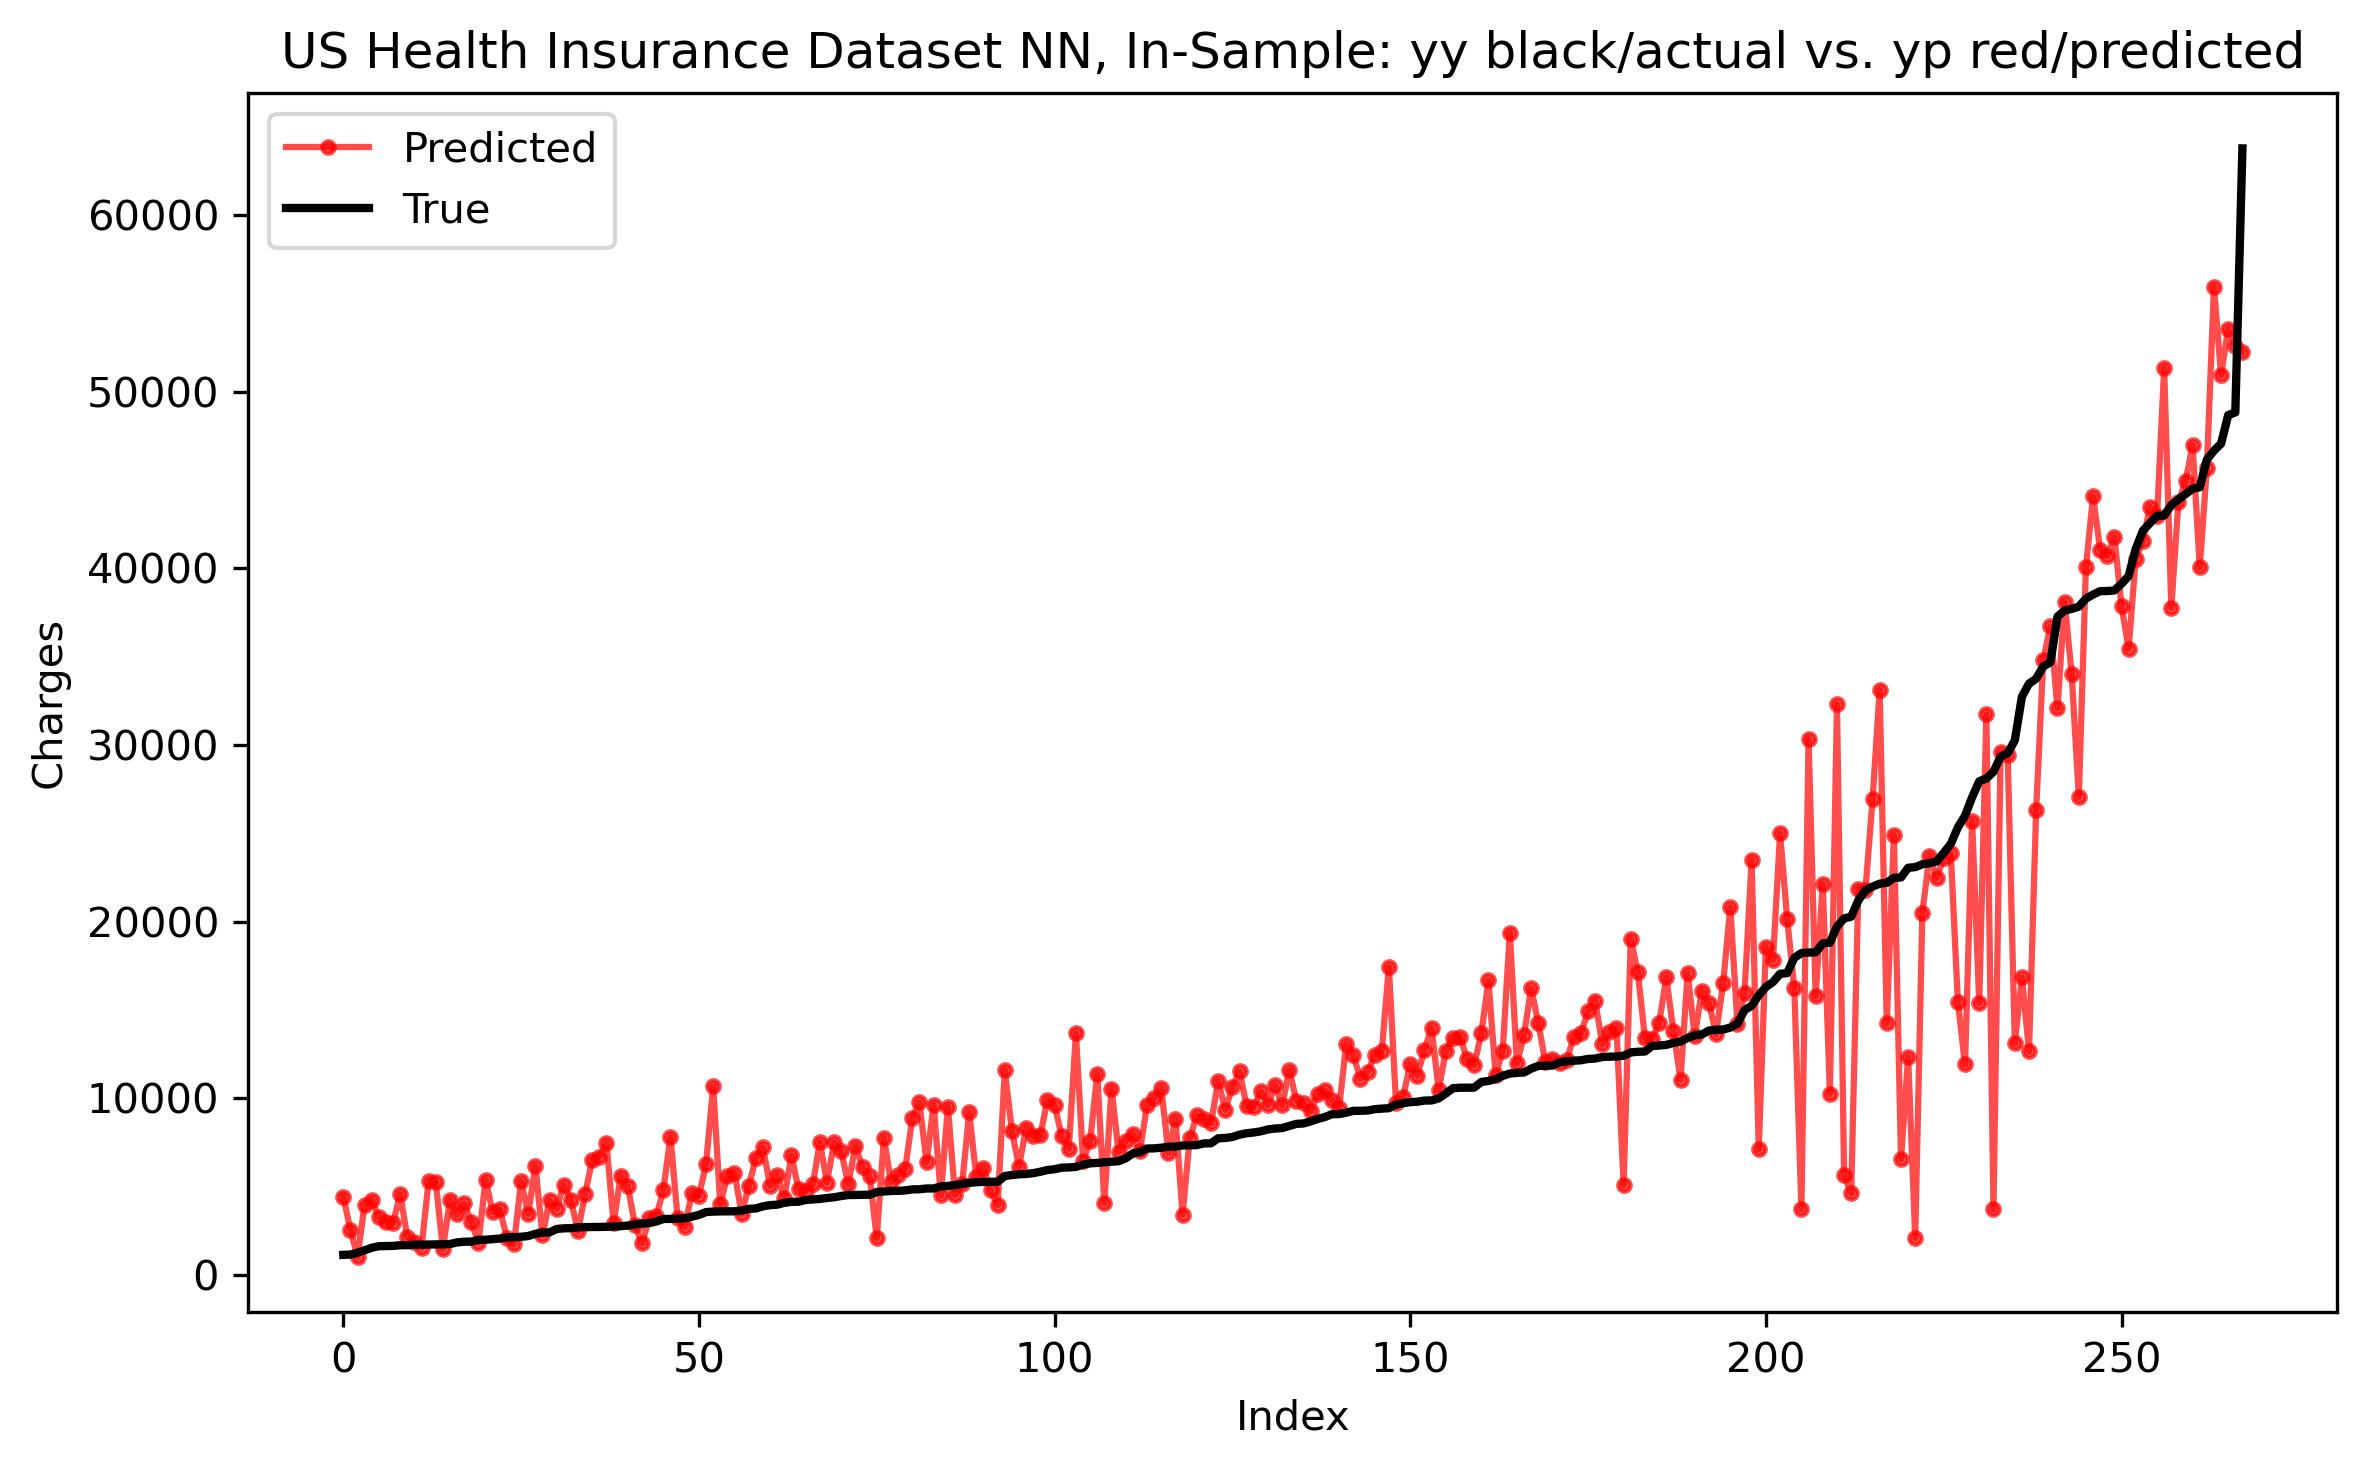
\includegraphics[width=0.9\textwidth]{figure/medical_out_sample_0.01.jpg}

\caption{Out-of-sample performance of a multi-layer neural network (Model 1) on the Insurance Charges dataset with a fine-tuned learning rate of $0.01$.}



\label{fig:cnn1}
\end{figure}

\end{document}